\documentclass[sigconf]{acmart}
\usepackage{amsmath}
\usepackage{lmodern}
\usepackage{graphicx}
\graphicspath{{./images/}}
\usepackage{caption}
\usepackage{subcaption}
\usepackage[notransparent]{svg}
\usepackage{hyperref}  % Added for hyperlink support


% Meta information
\title{Image “Outpainting” and Hole Filling: Final Report}
\subtitle{CS 5787 Deep Learning Final Project Report}

\author{Wentao Ye}
\email{wy335@cornell.edu}
\affiliation{%
  \institution{Cornell University}
  \city{New York}
  \state{New York}
  \country{USA}
}

\author{Mitchell Krieger}
\email{mak483@cornell.edu}
\affiliation{%
  \institution{Cornell University}
  \city{New York}
  \state{New York}
  \country{USA}
}

\author{Sebastian Jay}
\email{srj63@cornell.edu}
\affiliation{%
  \institution{Cornell University}
  \city{New York}
  \state{New York}
  \country{USA}
}

% Document begins
\begin{document}

\maketitle

\section*{Team Members}
Wentao Ye (wy335), Mitchell Krieger (mak483), Sebastian Jay (srj63)

\section*{Introduction}
This paper explores the relationship between image inpainting and outpainting by training a model capable of interpolating between two disparate images, blending them seamlessly into a single coherent scene. Inpainting, or image interpolation, is a computer vision task that aims to fill in missing or removed sections of an image, ensuring the completed area integrates smoothly with the existing content. Outpainting, or image extrapolation, generates extensions of an image beyond its original borders.

Drawing inspiration from both inpainting and outpainting, our objective is to generate a transitional region between two images. Traditional inpainting requires an understanding of the context and semantics surrounding the missing area to blend edges seamlessly into the original image. Outpainting, while sharing these challenges, has less context to infer from since it involves extending the image into an unknown space. Additionally, outpainting must handle long-range semantic dependencies, ensuring the generated extensions remain consistent with the original image no matter how far the extrapolation extends. Our task incorporates these challenges and introduces an added complexity: the need for the generated region to be semantically consistent with both images.

\section*{Related Work}
To address the challenges of our task, we leverage deep learning architectures capable of capturing both the semantics at the edges of each image and the relationships between regions across the two images. Historically, Convolutional Neural Networks (CNNs) have been widely used in vision tasks due to their efficiency and ability to learn spatial relationships \cite{LeCun1998, Krizhevsky2012}. However, CNNs have inherent limitations stemming from their design. Their architecture emphasizes locality, with weight sharing across the entire input, which makes them less adept at capturing long-range dependencies or relationships between non-local regions—a key requirement for complex tasks like ours.

Transformer-based architectures, particularly those employing attention mechanisms, have shown effectiveness in both inpainting and outpainting due to their capacity to model long-range dependencies. For example, \cite{Jiahui2018} demonstrated that incorporating a contextual attention layer significantly improved inpainting performance. Vision Transformers (ViTs) introduced by \cite{Dosovitskiy2020} expanded on this by applying self-attention mechanisms to computer vision tasks, enabling the modeling of global relationships in an image. Further advancements, such as Swin Transformers \cite{Liu2021}, refined the transformer architecture for vision tasks using hierarchical computation and shifted windows to improve efficiency and adaptability. These approaches, however, remain computationally expensive and require large datasets for effective training \cite{Dascoli2021}.

Yang et al. (2019) proposed a U-net GAN architecture to perform very long outpainting of a scene in one direction. They used Skip Horizontal Connections to connect each layer of the encoder and decoder in the Unet and an LSTM-based Recurrent Transfer Network to transfer the encoded sequences to the decoder. Using this method and generating in multiple steps, they were able to demonstrate long outpainting. Lu et al. (2021) expanded on this work by combining inpainting, outpainting, and image blending to fill in a scene between two images horizontally. They introduced a similar U-net GAN architecture to Yang et al. but also incorporated contextual attention and a Bidirectional Content Transfer module, which used LSTMs as a bottleneck to ensure spatial and semantic consistency across two images. Our work generalizes this approach by extending it to painting between two images in multiple directions.

\section*{Datasets}
We used the \textcolor{red}{\href{https://github.com/z-x-yang/NS-Outpainting}{NS-Outpainting}} dataset to train our models. It is used in the original U-Transformer paper. We also tested our trained model on additional images sourced from the internet.

\section*{Methods}

Our primary objective is to create a system that can generate a coherent transitional region between two images, effectively producing a seamless blend. The solution we propose combines insights from both inpainting and outpainting tasks. In particular, we aim to generalize the notion of completing missing image regions (inpainting) to a setting where the "hole" is defined by two non-overlapping image segments: one at the top-right corner and another at the bottom-left corner. By doing so, we effectively create a scenario where the model must understand and synthesize a large intermediate area that harmonizes with both input segments.

This section first outlines our overall framework and then discusses the detailed architecture of the generator and discriminator, our training procedure, and the loss functions used to ensure high-quality, contextually coherent image synthesis.

\subsection*{Overall Framework}

We frame our problem as learning a conditional generative model capable of taking two (possibly disparate) image patches as input and producing the missing middle region that stitches them together. While traditional inpainting models focus on filling small masked areas within a single image, we require the ability to fill a large gap that is spatially extended and semantically complex—one that must maintain coherence across potentially very different input segments.

In our approach, we rely on a Generative Adversarial Network (GAN) framework to produce plausible completions. The key intuition is that the discriminator will guide the generator to not only produce visually appealing local textures, but also maintain global consistency. We refine this idea by using a PatchGAN discriminator, which encourages detailed local realism, and a U-Net-based generator with skip connections to retain crucial spatial information.

Figure \ref{fig:general_process} shows the general high-level process of our method. Given two partial images—one cropped from the upper-right quadrant and another from the lower-left quadrant—we concatenate them along a predetermined boundary and feed the resulting partial image (with a large missing region in the center) into our generator. The generator synthesizes the missing portion, producing a final, coherent image. The discriminator then evaluates local patches of this completed image to ensure fidelity and realism.

\begin{figure}[h!]
    \centering
    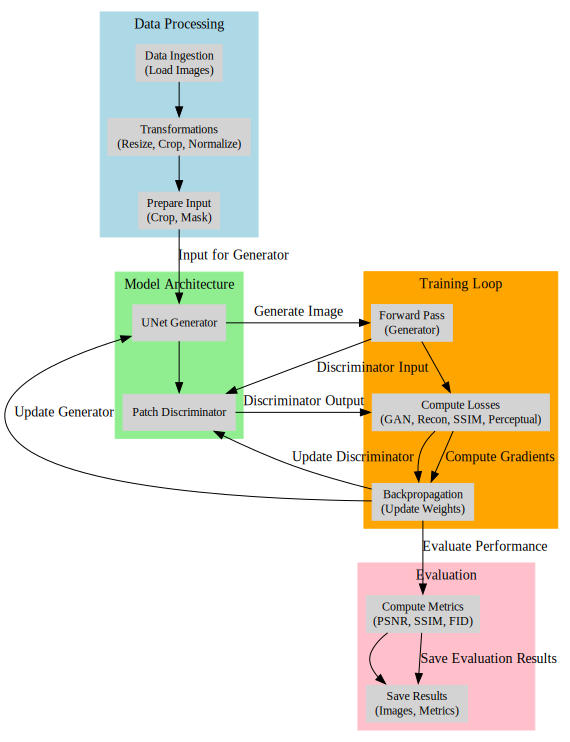
\includegraphics[width=\linewidth]{general_process.pdf}
    \caption{Overview of the general process. Two separate image patches (A and B) are combined with a large missing region in the center. Our system synthesizes a realistic, coherent image that bridges the gap between these two input patches.}
    \label{fig:general_process}
\end{figure}

\subsection*{Generator Architecture}

\noindent\textbf{U-Net-based Generator:}  
Our generator is inspired by the U-Net architecture, originally introduced for biomedical image segmentation \cite{Ronneberger2015}. The U-Net design is well-suited to our task because it uses a symmetric encoder-decoder structure with skip connections that maintain spatial details. The encoder progressively extracts increasingly abstract and semantically rich features, while the decoder gradually reconstructs the image, guided by skip connections that help preserve local structure and high-frequency details lost in downsampling.

Unlike traditional U-Nets used in segmentation, our generator must handle a complex conditional input: a partially completed scene with missing sections. We adapt the network to take in our concatenated partial images and to output a completed image of the same size. The final layer of the generator uses a Tanh activation, ensuring that output values lie in the range $[-1, 1]$ to match the normalized input image range.

Figure \ref{fig:generator} illustrates the architecture of our U-Net generator. On the left, we show the downsampling path, which encodes the input into a deep latent representation. On the right, the corresponding upsampling path decodes this latent representation back into a full-resolution image, with skip connections bridging corresponding layers.

\begin{figure}[h!]
    \centering
    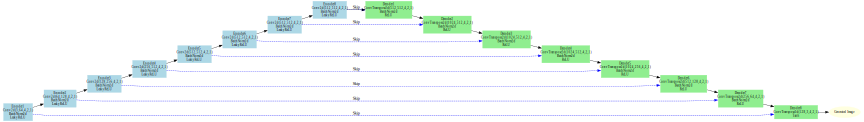
\includegraphics[width=\linewidth]{generator.pdf}
    \caption{The U-Net-based generator architecture. The input is fed into a series of convolutional layers that progressively downsample and extract features, and then the decoded representations are combined with earlier features through skip connections to produce the final completed image.}
    \label{fig:generator}
\end{figure}

\subsection*{Discriminator Architecture}

\noindent\textbf{PatchGAN Discriminator:}  
A traditional image-level discriminator that outputs a single scalar value for real/fake judgment can sometimes ignore subtle local details. To encourage the model to produce high-quality textures and local patterns, we adopt a PatchGAN discriminator \cite{Isola2017}. Instead of a single output, the PatchGAN outputs an $N \times N$ grid of values, each corresponding to the realism of a local patch in the image. This design is known to better capture local style and texture, and it prevents the generator from focusing only on global structure at the expense of local detail.

Our PatchGAN discriminator takes the generated or real completed images as input and classifies each patch as real or fake. This encourages the generator to produce realistic local details throughout the image, not just to fool a global classifier. Figure \ref{fig:discriminator} shows the schematic of our PatchGAN discriminator. It progressively downsamples the input image through convolutional layers until the spatial resolution matches that of the patch-based output. Each output value corresponds to the authenticity of a small local region of the image.

\begin{figure}[h!]
    \centering
    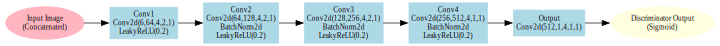
\includegraphics[width=\linewidth]{images/discriminator.pdf}
    \caption{The PatchGAN discriminator architecture. It classifies overlapping patches of the image, encouraging the generator to produce realistic local textures and details.}
    \label{fig:discriminator}
\end{figure}

\subsection*{Training Procedure}

\noindent\textbf{Adversarial Training:}  
We train our model following the adversarial learning paradigm. During training, the generator ($G$) receives two partial images and attempts to complete the missing region. The discriminator ($D$) then tries to distinguish the real, fully combined images from the synthetic outputs. We adopt a least-squares GAN (LSGAN) formulation \cite{Mao2017} for stable training. The generator’s goal is to produce samples that the discriminator classifies as real, while the discriminator aims to differentiate between real and generated samples accurately.

Our training alternates between optimizing $D$ and $G$. By iteratively improving both models, we steer the generator toward producing outputs that appear increasingly like the ground-truth combined images, balancing local detail with global coherence.

\noindent\textbf{Implementation Details:}  
We implement our model using PyTorch. The input images are normalized to $[-1, 1]$. The optimizer used is Adam \cite{Kingma2015} with a learning rate of $2 \times 10^{-4}$, $\beta_1 = 0.5$, and $\beta_2 = 0.999$. We train our models on a single GPU, and regularly monitor training by evaluating intermediate outputs to ensure visual plausibility. Model checkpoints are saved periodically.

\subsection*{Loss Functions}

\noindent\textbf{Adversarial Loss:}  
For the adversarial part, we use the least-squares objective:
\[
\mathcal{L}_{\text{GAN}} = \mathbb{E}[(D(x)-1)^2] + \mathbb{E}[D(G(x))^2],
\]
where $x$ denotes the real completed image and $G(x)$ is the generator’s output given partial input.

\noindent\textbf{Reconstruction Loss (L1 Loss):}  
To ensure that the generated regions closely approximate the ground truth, we use an L1 reconstruction loss on the masked area:
\[
\mathcal{L}_{\text{recon}} = \| x - G(x) \|_1.
\]

\noindent\textbf{Structural Similarity (SSIM) Loss:}  
Beyond pixel-level accuracy, we incorporate an SSIM loss to encourage structural fidelity:
\[
\mathcal{L}_{\text{SSIM}} = 1 - \text{SSIM}(x, G(x)),
\]
where $\text{SSIM}(\cdot,\cdot)$ measures perceptual similarity.

\noindent\textbf{Perceptual Loss:}  
We also use a perceptual loss, computed from features of a pre-trained VGG-19 network \cite{Johnson2016}, to ensure that the synthesized regions align with the high-level semantics of the original scenes:
\[
\mathcal{L}_{\text{perc}} = \sum_{l} \| \phi_l(x) - \phi_l(G(x)) \|_2,
\]
where $\phi_l(\cdot)$ is the feature map at layer $l$ of VGG-19.

\noindent\textbf{Combined Objective:}  
Our final generator objective combines these terms:
\[
\mathcal{L}_{G} = \mathcal{L}_{\text{GAN}}(G,D) + \lambda_{\text{recon}}\mathcal{L}_{\text{recon}}(G) + \lambda_{\text{SSIM}}\mathcal{L}_{\text{SSIM}}(G) + \lambda_{\text{perc}}\mathcal{L}_{\text{perc}}(G),
\]
with weights $\lambda_{\text{recon}}$, $\lambda_{\text{SSIM}}$, and $\lambda_{\text{perc}}$ controlling the importance of each component.

\subsection*{Alternative Approaches Considered}

We also considered transformer-based methods and diffusion-based inpainting models, inspired by recent work in long-range dependency modeling. However, these approaches typically require extensive computational resources and large training datasets to achieve high-quality results. For instance, Vision Transformers (ViTs) or transformer-based architectures excel at capturing global dependencies, but training them from scratch on our dataset proved challenging and computationally expensive.

Likewise, diffusion-based models are known for their high-quality samples, but training a diffusion inpainting model from scratch is computationally intensive and can struggle without massive training resources. By contrast, our proposed GAN-based approach with a U-Net generator and PatchGAN discriminator yields plausible results more efficiently, making it a practical solution within our computational constraints.

\subsection*{Justification of Approach}
Our implementation uses PyTorch, and we normalize inputs to the $[-1, 1]$ range. The models are trained using the Adam optimizer (Kingma \& Ba, 2015) with a learning rate of $2 \times 10^{-4}$ and $\beta_1 = 0.5$, $\beta_2 = 0.999$. We periodically save model checkpoints and evaluate intermediate outputs to ensure that the generator’s outputs become progressively more realistic and semantically meaningful. 

Our chosen approach strikes a balance between complexity, computational feasibility, and output quality. The U-Net generator ensures that spatial details and global coherence are preserved, while the PatchGAN discriminator encourages realistic local texture synthesis. The combination of reconstruction, SSIM, and perceptual losses helps produce both structurally consistent and perceptually convincing completions. Although state-of-the-art pretrained diffusion or transformer-based models could, in theory, produce even more photorealistic results, our method achieves a strong baseline performance with significantly fewer computational resources, making it suitable for a wide range of applications and research settings.

\section*{Experiments}

\subsection*{Experimentation Steps}

We completed the following steps when experimenting on our models, sometimes stopping early and not completing all steps if we did not see comparable results to our previous work:

\begin{enumerate}
    \item \textbf{Training:} As explained above, we removed the upper right and lower left quadrants of each training image and computed loss metrics on the model’s prediction of the original intact image without any quadrants removed. We then computed metrics on the test set by evaluating the model’s prediction of the uncropped test set images, using cropped test set images with their upper right and lower left quadrants removed as input.
    
    \item \textbf{Visual inspection of results on the same cropped input image:} Before computing metrics, we visually inspected each model’s outputs when computing predictions from the test set. When this step yielded low or unrecognizable resemblance to the input image, we stopped and revised the model.
    
    \item \textbf{Metrics computation:} We computed the Peak Signal-to-Noise (PSNR), Structural Similarity Index Measure (SSIM), and Fréchet Inception Distance (FID) metrics for each model on the test images.
    
    \item \textbf{Visual inspection of results on two different cropped input images:} In contrast to step 2, where we used two quadrants of the same image, here we used the upper right quadrant of one image and the lower left quadrant of a different image as input to the model and visually inspected the resulting completed image of an intact scene.
    
    \item \textbf{Visual inspection with larger cropping mask of one input image:} Here we repeated step 2, but instead of using the entire lower left quadrant and the entire upper right quadrant as input (which meet at the center of the image), we only used the bottom left portion of the lower left quadrant and the upper right portion of the upper right quadrant, which do not meet in any part of the image.
    
    \item \textbf{Visual inspection with larger cropping mask of two different images:} Here we used a larger mask as in step 5 on two distinct images of different scenes, as in step 4.
\end{enumerate}

We trained and tested all of our models on the NS-Outpainting dataset containing wide panoramic images of scenery. Some example images from it are shown below:

\begin{figure}[h!]
    \centering
    \includegraphics[width=\linewidth]{ns_dataset}
    \caption{Example images from the NS-Outpainting dataset that we used to train our models.}
    \label{fig:ns_dataset}
\end{figure}

\subsection*{Models}

We experimented with the following models:

U-Transformer model: here we sought to replicate the results achieved by Gao et al in the “Generalised Image Outpainting with U-Transformer” paper. We completed experimentation steps 1-2 for this model as a reference point, but found that achieving results comparable to that of the paper was computationally infeasible with our resources.

\begin{figure}[h!]
    \centering
    \includegraphics[width=\linewidth]{u_transformer}
    \caption{Output from the U-Transformer model, to paint outwards from the original image. Note that this is not the same task as we are attempting to complete with our models.}
    \label{fig:u_transformer}
\end{figure}

The first diffusion model that we tried was inspired by the “Repaint” diffusion model published by Lugmayr et al in the paper “RePaint: Inpainting using Denoising Diffusion Probabilistic Models”. The architecture is shown here:

\begin{figure}[h!]
    \centering
    \includegraphics[width=\linewidth]{repaint_architecture}
    \caption{Illustration of our model's architecture that was based on the RePaint diffusion model architecture.}
    \label{fig:repaint_architecture}
\end{figure}

And our output from using this model is shown below:

\begin{figure}[h!]
    \centering
    \includegraphics[width=\linewidth]{repaint_results}
    \caption{Output from the RePaint model that we tried.}
    \label{fig:repaint_results}
\end{figure}

However, we realized after producing these output images that there was some leakage from the training data into the test data. Hence, we do not consider this to be a valid result.

Our best independently developed result was achieved with our GAN model, which uses the PatchGAN discriminator and UNet generator as described in greater detail above.

Below are some of the results that we achieved using the GAN model on our test set of images, when the model received one cropped image of the same scene as input (i.e. step 2 in the list of “Experimentation Steps” above):

\begin{figure}[h!]
    \centering
    \includegraphics[width=\linewidth]{gan_step_2}
    \caption{Results from experimentation step 2 of our final GAN model}
    \label{fig:gan_step_2}
\end{figure}

Here are the metrics that we achieved with our GAN model, using the outputs from step 2 in our list of “Experimentation Steps” above:

\begin{figure}[h!]
    \centering
    \includegraphics[width=\linewidth]{gan_metrics}
    \caption{Metrics achieved by our final GAN model on the test set of images, as described in experimentation step 2.}
    \label{fig:gan_metrics}
\end{figure}

Below are some of the results that we achieved using the GAN model on our test set of images, when the model received two adjacent and distinct images of different scenes as input, each cropped to only contain one quadrant (i.e. step 4 in the list of “Experimentation Steps” above):

\begin{figure}[h!]
    \centering
    \includegraphics[width=\linewidth]{gan_step_4}
    \caption{Results outputted by our final GAN model from input images of two separate scenes, as described in experimentation step 4.}
    \label{fig:gan_step_4}
\end{figure}

We tried repeatedly to train a non-pretrained diffusion model from scratch but were unable to achieve visually satisfactory results with it. Here are some examples of what it produced in step 2:

\begin{figure}[h!]
    \centering
    \includegraphics[width=\linewidth]{diffusion_step_2_1}
    \caption{Example 1: our non-pretrained diffusion model output from Experimentation Step 2.}
    \label{fig:diffusion_step_2_1}
\end{figure}

\begin{figure}[h!]
    \centering
    \includegraphics[width=\linewidth]{diffusion_step_2_2}
    \caption{Example 2: our non-pretrained diffusion model output from Experimentation Step 2.}
    \label{fig:diffusion_step_2_2}
\end{figure}

\begin{figure}[h!]
    \centering
    \includegraphics[width=\linewidth]{diffusion_step_2_3}
    \caption{Example 3: our non-pretrained diffusion model output from Experimentation Step 2.}
    \label{fig:diffusion_step_2_3}
\end{figure}

\begin{figure}[h!]
    \centering
    \includegraphics[width=\linewidth]{diffusion_step_2_4}
    \caption{Example 4: our non-pretrained diffusion model output from Experimentation Step 2.}
    \label{fig:diffusion_step_2_4}
\end{figure}

\begin{figure}[h!]
    \centering
    \includegraphics[width=\linewidth]{diffusion_step_2_5}
    \caption{Example 5: our non-pretrained diffusion model output from Experimentation Step 2.}
    \label{fig:diffusion_step_2_5}
\end{figure}

Finally, here are some of the results that we achieved using the GAN model on our test set of images, when the model received two non-adjacent distinct images of different scenes as input, each cropped more extensively to contain only part of one quadrant (i.e. step 6 in the list of “Experimentation Steps” above):

\begin{figure}[h!]
    \centering
    \includegraphics[width=\linewidth]{gan_step_6}
    \caption{Our final GAN model's output in experimentation step 6, using non-adjacent images of disparate scenes.}
    \label{fig:gan_step_6}
\end{figure}

As a comparison benchmark, we also tried a pre-trained Stable Diffusion model from huggingface. Example results from steps 2 and 5 are shown below:

\begin{figure}[h!]
    \centering
    \includegraphics[width=\linewidth]{stable_diffusion_step_2_1}
    \caption{Example 1: pretrained Stable Diffusion model output from Experimentation Step 2.}
    \label{fig:stable_diffusion_step_2_1}
\end{figure}

\begin{figure}[h!]
    \centering
    \includegraphics[width=\linewidth]{stable_diffusion_step_2_2}
    \caption{Example 2: pretrained Stable Diffusion model output from Experimentation Step 2.}
    \label{fig:stable_diffusion_step_2_2}
\end{figure}

\begin{figure}[h!]
    \centering
    \includegraphics[width=\linewidth]{stable_diffusion_step_5}
    \caption{Example 1: pretrained Stable Diffusion model output from Experimentation Step 5.}
    \label{fig:stable_diffusion_step_5}
\end{figure}

\section*{Conclusion}

As can be seen from the images above, the best results that we achieved from a model that we developed were obtained from our final GAN model, which integrates a U-Net-based generator and a PatchGAN-based discriminator.

Notably, the state of the art pretrained Stable Diffusion model \textit{“was trained using 256 Nvidia A100 GPUs on Amazon Web Services for a total of 150,000 GPU-hours, at a cost of \$600,000.”} By contrast, we achieved the results shown above with our GAN model after training for just 5 hours on a RTX 2070. We’d love to see what our final GAN model can achieve with a training budget of \$600,000!

\section*{Appendix}

All of our code can be found in \textcolor{red}{\href{https://github.com/yewentao256/CS5787-Final}{our repository}} on Github.

\begin{thebibliography}{9}
    \bibitem{Dascoli2021} Stéphane d’Ascoli et al., "ConViT: Improving Vision Transformers with Soft Convolutional Inductive Biases," \textit{CVPR 2021}, 2021.
    \bibitem{Dosovitskiy2020} A. Dosovitskiy, et al., "Discriminative Unsupervised Feature Learning with Exemplar Convolutional Neural Networks," \textit{IEEE Transactions on Pattern Analysis and Machine Intelligence}, 2020.
    \bibitem{Gao2022} Penglei Gao et al., "Generalised Image Outpainting with U-Transformer," \textit{CVPR 2022}.
    \bibitem{Isola2017} P. Isola, et al., "Image-to-Image Translation with Conditional Adversarial Networks," \textit{CVPR 2017}.
    \bibitem{Jiahui2018} J. Yang, et al., "Contextual Attention for Image Inpainting," \textit{CVPR 2018}.
    \bibitem{Krizhevsky2012} A. Krizhevsky, et al., "ImageNet Classification with Deep Convolutional Neural Networks," \textit{NIPS 2012}.
    \bibitem{LeCun1998} Y. LeCun, et al., "Gradient-Based Learning Applied to Document Recognition," \textit{Proceedings of the IEEE}.
    \bibitem{Liu2021} Z. Liu, et al., "Swin Transformer: Hierarchical Vision Transformer Using Shifted Windows," \textit{ICCV 2021}.
    \bibitem{Lu2021} Chia-Ni Liu, et al., "Bridging the Visual Gap: Wide-Range Image Blending," \textit{CVPR 2021}.
    \bibitem{Lugmayr2022} Andreas Lugmayr, et al., "RePaint: Inpainting Using Denoising Diffusion Probabilistic Models," \textit{CVPR 2022}.
    \bibitem{Mao2017} X. Mao, et al., "Least Squares Generative Adversarial Networks," \textit{ICCV 2017}.
    \bibitem{Mostaque2022} @EMostaque on Twitter, "The Stable Diffusion model was trained using 256 Nvidia A100 GPUs on Amazon Web Services for a total of 150,000 GPU-hours, at a cost of \$600,000." \textit{https://twitter.com/EMostaque/status/1509780730730734592}
    \bibitem{Rombach2022} Robin Rombach, et al., "High-Resolution Image Synthesis with Latent Diffusion Models," \textit{CVPR 2022}.
    \bibitem{Tang2024} Luming Tang, et al., "RealFill: Reference-Driven Generation for Authentic Image Completion," \textit{SIGGRAPH 2024}.
    \bibitem{Yang2019} Zongxin Yang, et al., "Very Long Natural Scenery Image Prediction by Outpainting," \textit{ICCV 2019}.
    \bibitem{Yu2018} Jiahui Yu et al., "Generative Image Inpainting with Contextual Attention," \textit{CVPR 2018}.
\end{thebibliography}

\end{document}
